\documentclass[12pt, leqno]{article}
\usepackage[english,russian]{babel}
\usepackage{fontspec}
\usepackage[utf8]{inputenc}
\usepackage{epigraph}
\usepackage{tabularx}
\usepackage[leqno]{amsmath}
\setmainfont{Times New Roman}
\setlength\parindent{0pt}
\usepackage[colorlinks=true,urlcolor=blue]{hyperref}        
\usepackage{minted} 
\usepackage[xetex,final]{graphicx}
\usepackage{float}%"Плавающие" картинки
\usepackage{wrapfig}%Обтекание фигур (таблиц, картинок и прочег
\usepackage{epstopdf}
 
\begin{document}

\section*{Арифметичсекая прогрессия. Рекурсия}
\begin{flushleft}
\textbf{Вопросы рекурсии:} Рекурентные формулы и реализация
\end{flushleft}

Арифмети́ческая прогре́ссия — числовая последовательность вида: 

\begin{equation}
a_{1},\ a_{1}+d,\ a_{1}+2d,\ \ldots ,\ a_{1}+(n-1)d,\ \ldots \ ,
\end{equation}

рекурентная форму имеет вид:


\begin{equation}
a_{n}=a_{n-1}+d
\end{equation}

Общий член арифметической прогрессии
\begin{equation}
a_{n}=a_{1}+(n-1)d 
\end{equation}

\begin{equation}
a_{n}=a_{m}-(m-n)d
\end{equation}

Сумма первых $ n $ членов арифметической прогрессии  
$ S_{n}=\sum _{i=1}^{n}a_{i}=a_{1}+a_{2}+\ldots +a_{n} $ 
может быть найдена по формулам: 

\begin{equation}
S_{n}={\dfrac {a_{1}+a_{n}}{2}}\cdot n 
\end{equation}

Дальше можно смотреть по ссылке:

\href{https://ru.wikipedia.org/wiki/Арифметическая_прогрессия}{Арифметическая прогрессия}


\clearpage 

\noindent Образец кода на лисп (sbcl):  
 
\begin{minted}[fontsize=\small]{lisp}

;;;; Arithmetic Progression
(defconstant s 7 "cooef")

;; https://ru.wikipedia.org/wiki/Арифметическая_прогрессия

;;; This function recursively build pregression
(defun arithmeticProgression (summ n)
(
;;Count 'cond'-ition statement"                 
    cond ((<= n 0 ) nil)
         (t (cons ( + summ  s)  (arithmeticProgression (  + summ  s ) (- n 1)))) 
    )
)

(defun cli/parameter()
;; Get command line argument" 
    (let (
        (args sb-ext:*posix-argv*))
        (car (cdr args)))
)

;; main print
;; input   ./arithmetic_progression.lisp  <n = 7>
(defun main()
(terpri)
(time (
       format T "~a  SUMM = ~d"
          (arithmeticProgression 0 (- ( parse-integer (cli/parameter)) 1))
          (apply '+ (arithmeticProgression 0 (- ( parse-integer (cli/parameter)) 1) ))
          )))

(main)


\end{minted}  

\clearpage 
Ниже представлен результат для $ n = 7$

\begin{figure}[h]
\center{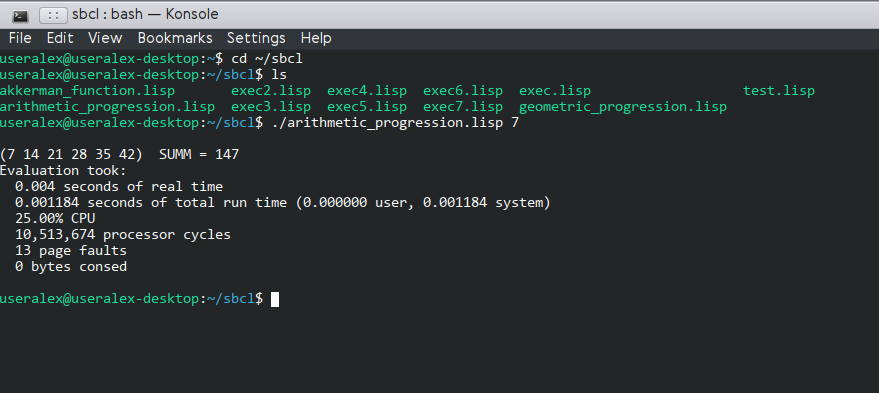
\includegraphics[width=0.8\textwidth,natwidth=610,natheight=642]{./img/Screenshot_20250113_143457.png}}
\caption{Скриншот вывода нашего скрипта}
\label{ris:image}
\end{figure}

  

\end{document}